% generated by make_figures.py tiles (factor_tiles.write_tex); do not edit
\newcommand{\tilegrid}{%
\begin{table*}[p]
\captionsetup{type=figure}
\centering
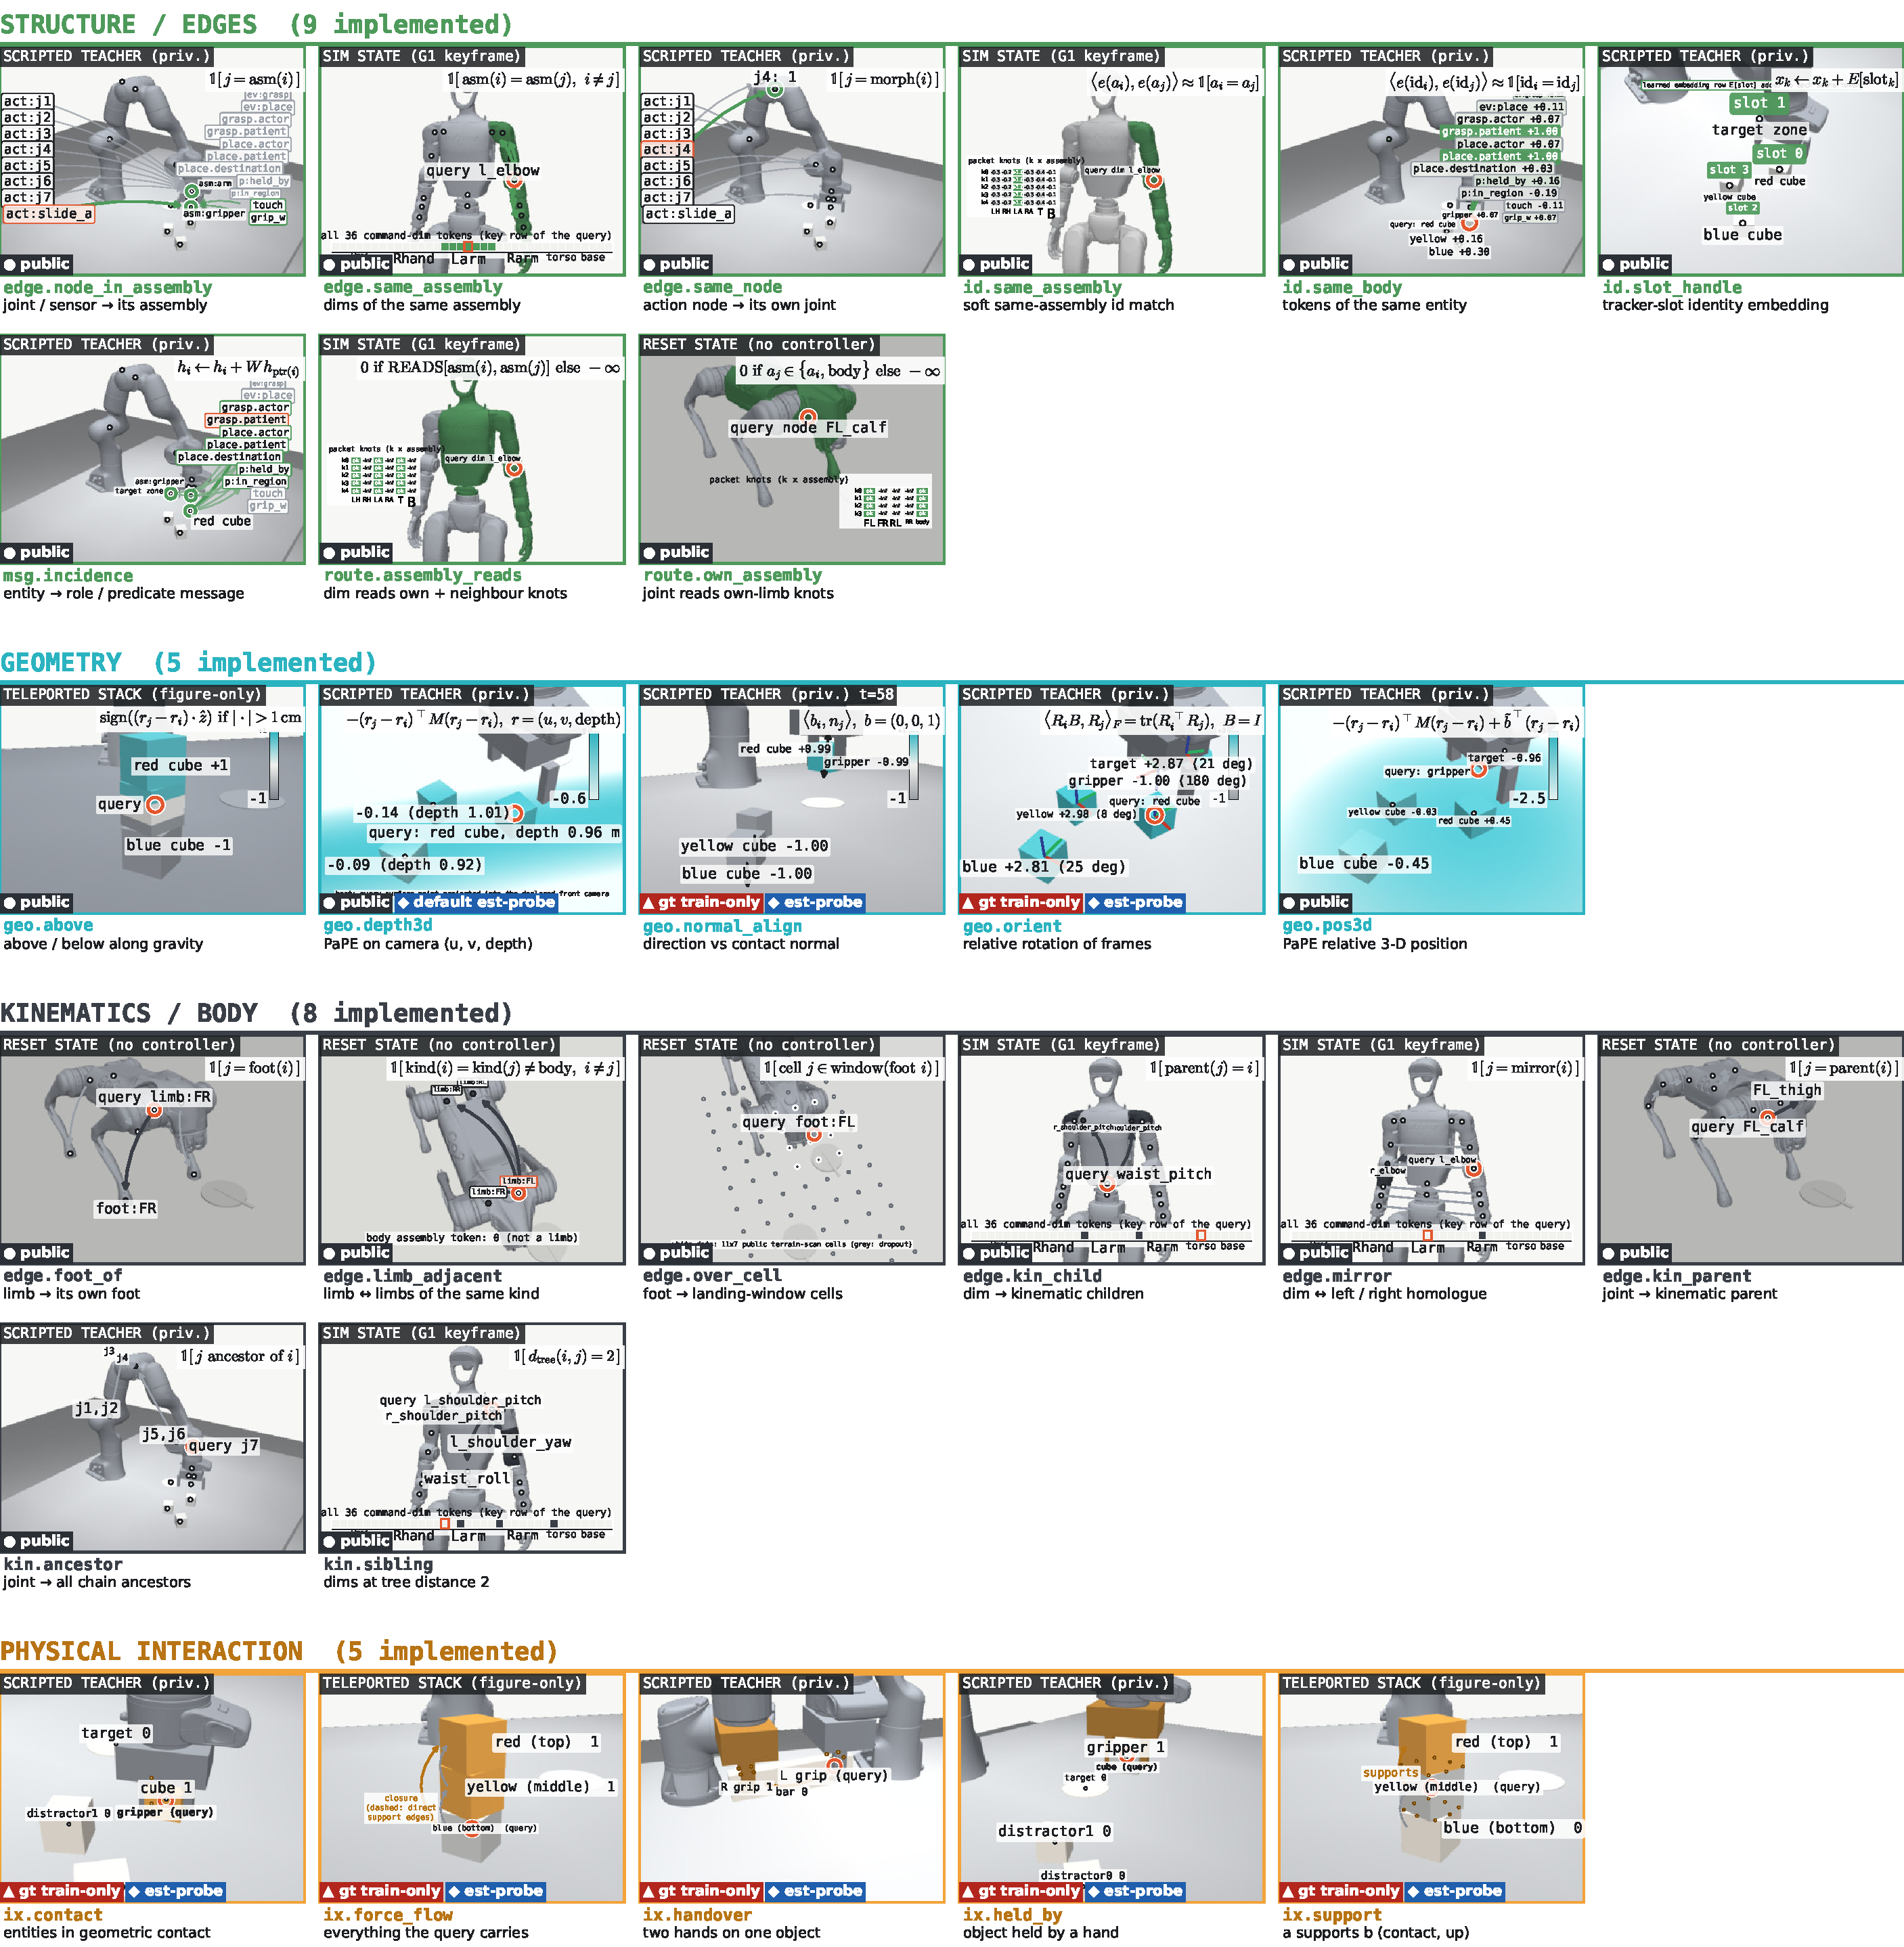
\includegraphics[width=\textwidth]{figures/factor_grid_p1.pdf}
\captionsetup{font=footnotesize}\caption{\textbf{Every implemented relation factor, one tile each} (75 tiles on 5 pages, families in the row order of Table~\ref{tab:relations}). Each tile shows one factor's term for one query token (ring or outlined chip) on a real simulator or environment state, computed by the repository's factor operators or label code; \emph{nothing is trained attention or a trained probe output}. Frame colour = family (Fig.~\ref{fig:fig2}'s four plus structure green); probe readouts are coloured by what they encode (cyan a geometric quantity, amber physical interaction, violet task/procedure state). Top-left chip: scene source (\textsc{scripted teacher} states are privileged). Bottom badge: term source. \emph{public (given)}: computed from public inputs, deployable as shown; \emph{estimated-probe}: the deployed term is the probe's estimate (not shown); \emph{gt \ldots\ training-only}: the colour is the simulator-truth label that trains that probe or readout, never a deployed input. Learned coefficients (edge weights $w$, PaPE $a,b$, rotation/alignment coefficients, same-code gain, task gate) are \emph{set by hand} and stated on the tile. \textsc{illustrative}: \texttt{edge.support\_of} uses a figure-only task-graph variant (no shipped arm/dual graph binds a support role to an entity); \texttt{probe.psi0.grasp\_pt} / \texttt{grasp\_face} show a real replay frame without a label (the replays carry no contact positions). Under each tile: factor, what it encodes, operator and form, source. Generated by \texttt{make\_figures.py tiles}.}\label{fig:tiles}
\end{table*}
\begin{table*}[p]
\captionsetup{type=figure}
\centering
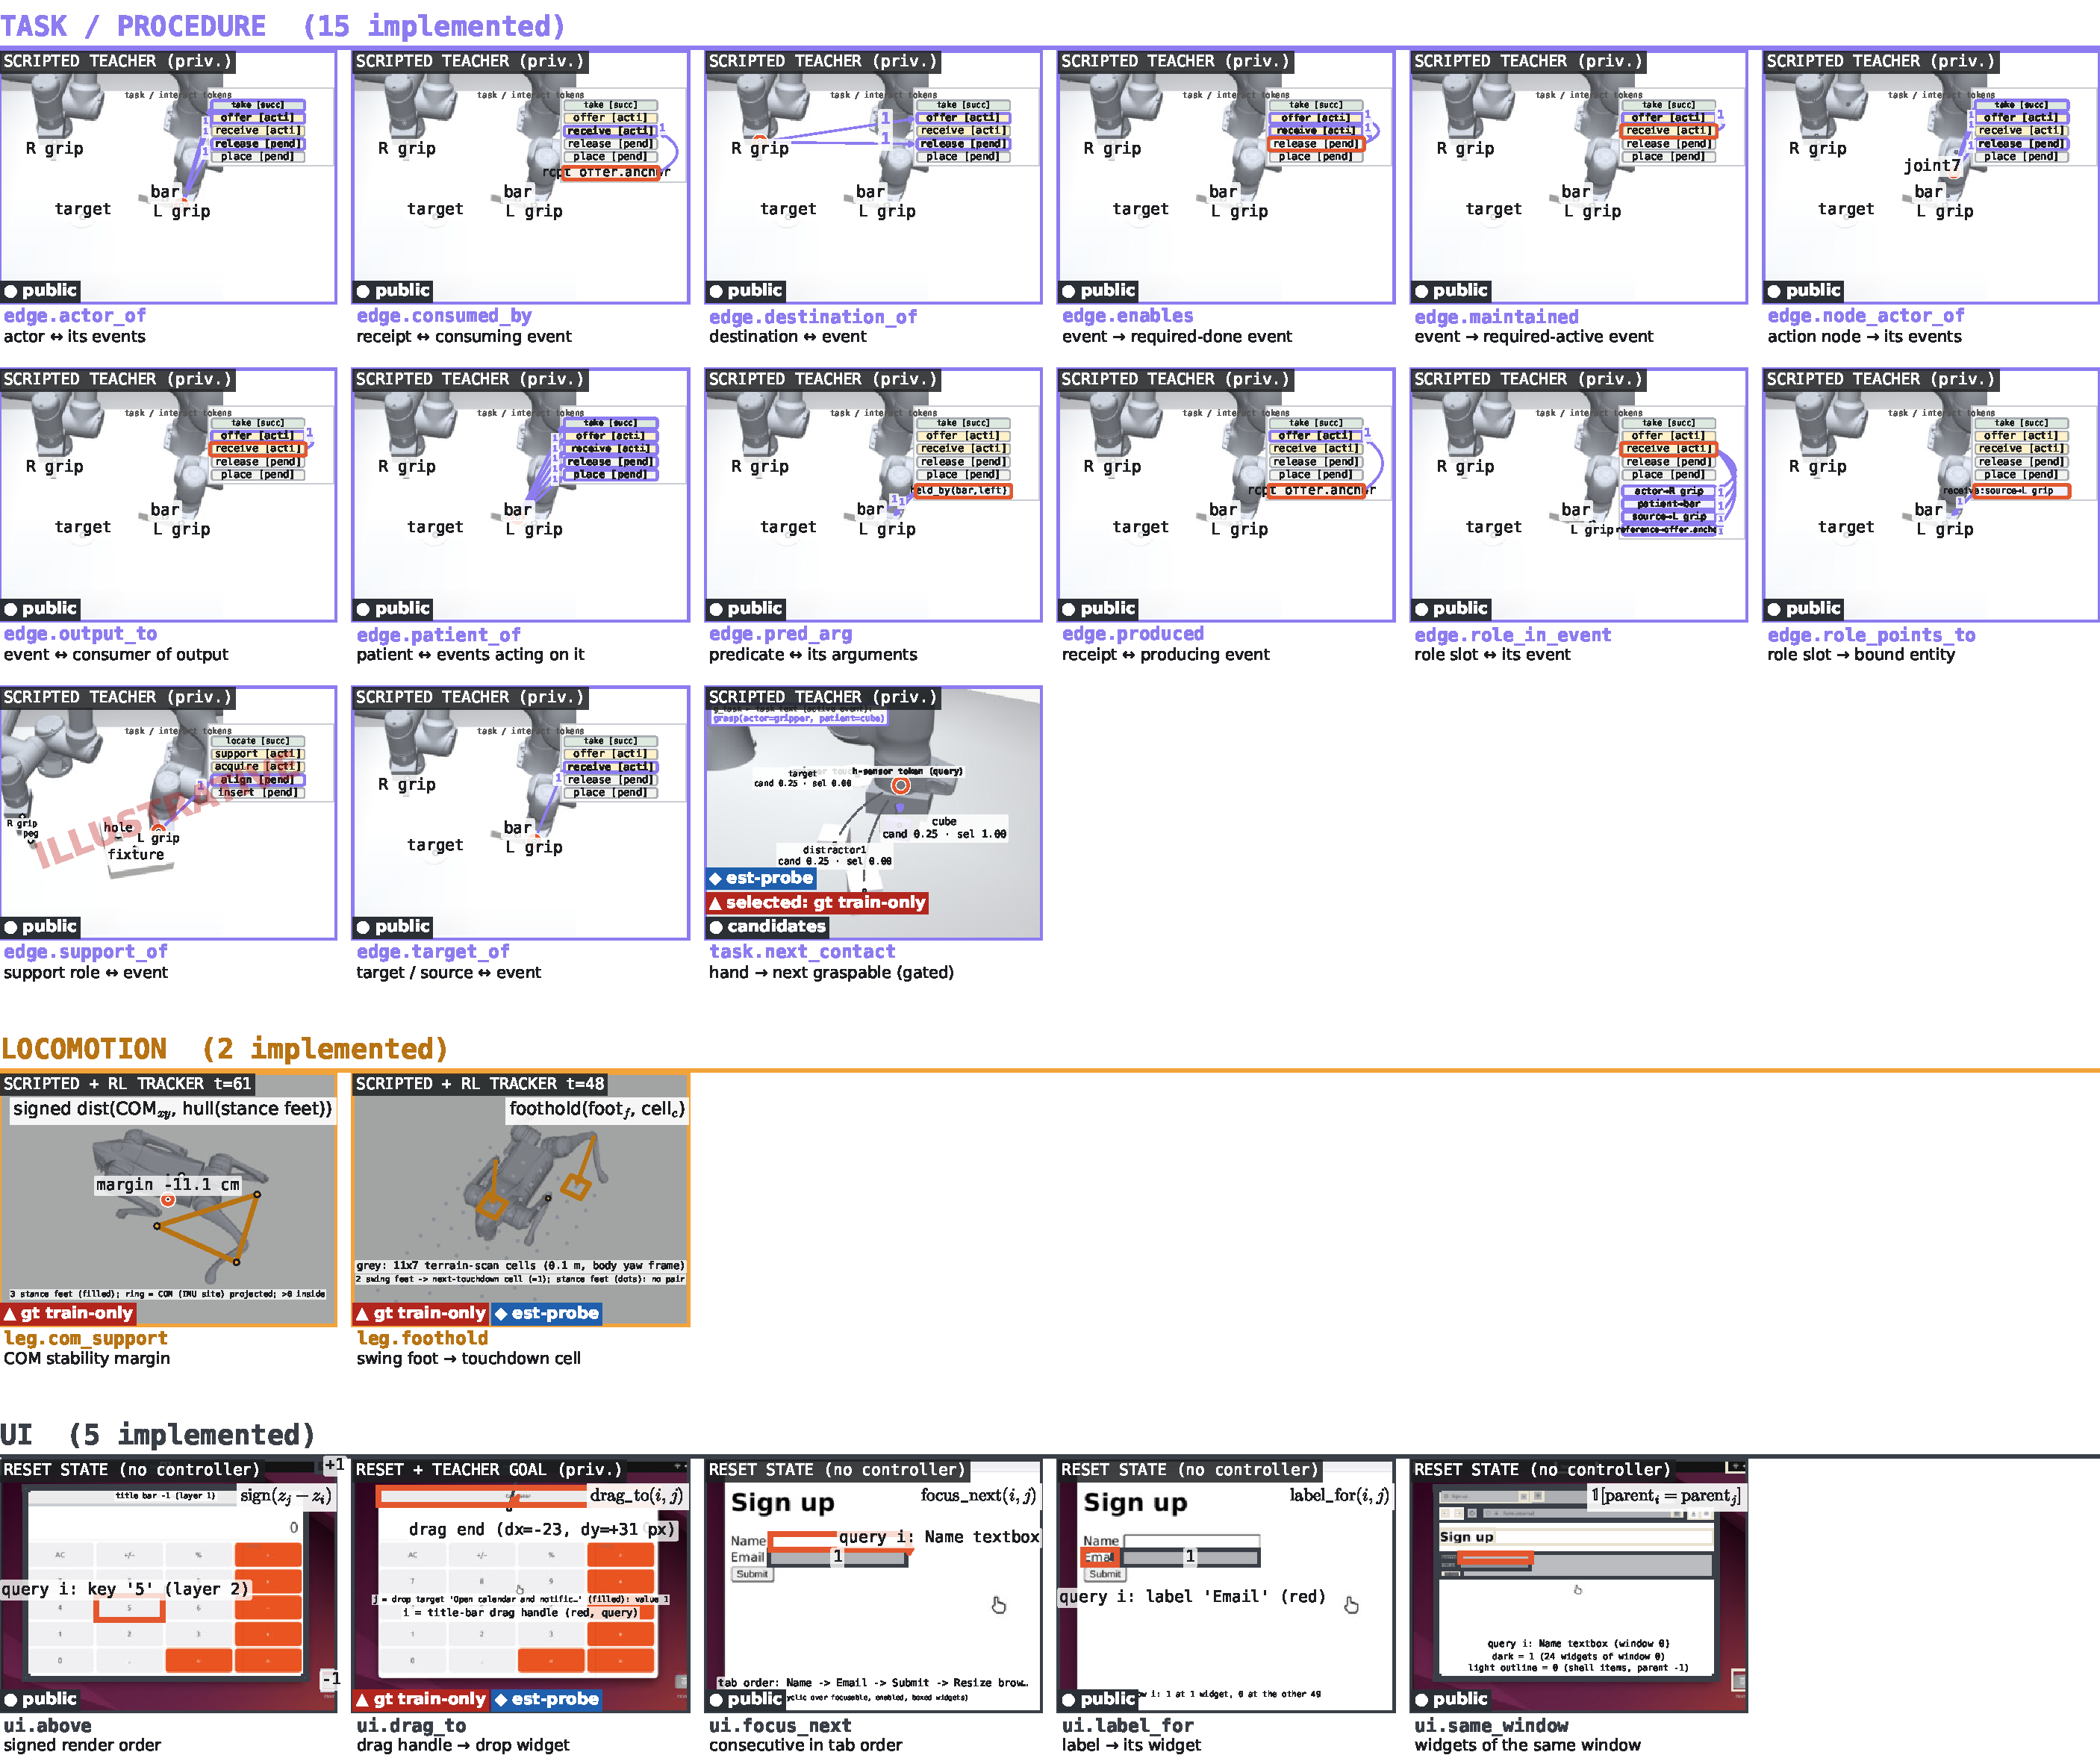
\includegraphics[width=\textwidth]{figures/factor_grid_p2.pdf}
\ContinuedFloat\captionsetup{font=footnotesize}\caption[]{\textbf{Every implemented relation factor} (continued, page 2/5). Badges, colours and marks as on the first page.}
\end{table*}
\begin{table*}[p]
\captionsetup{type=figure}
\centering
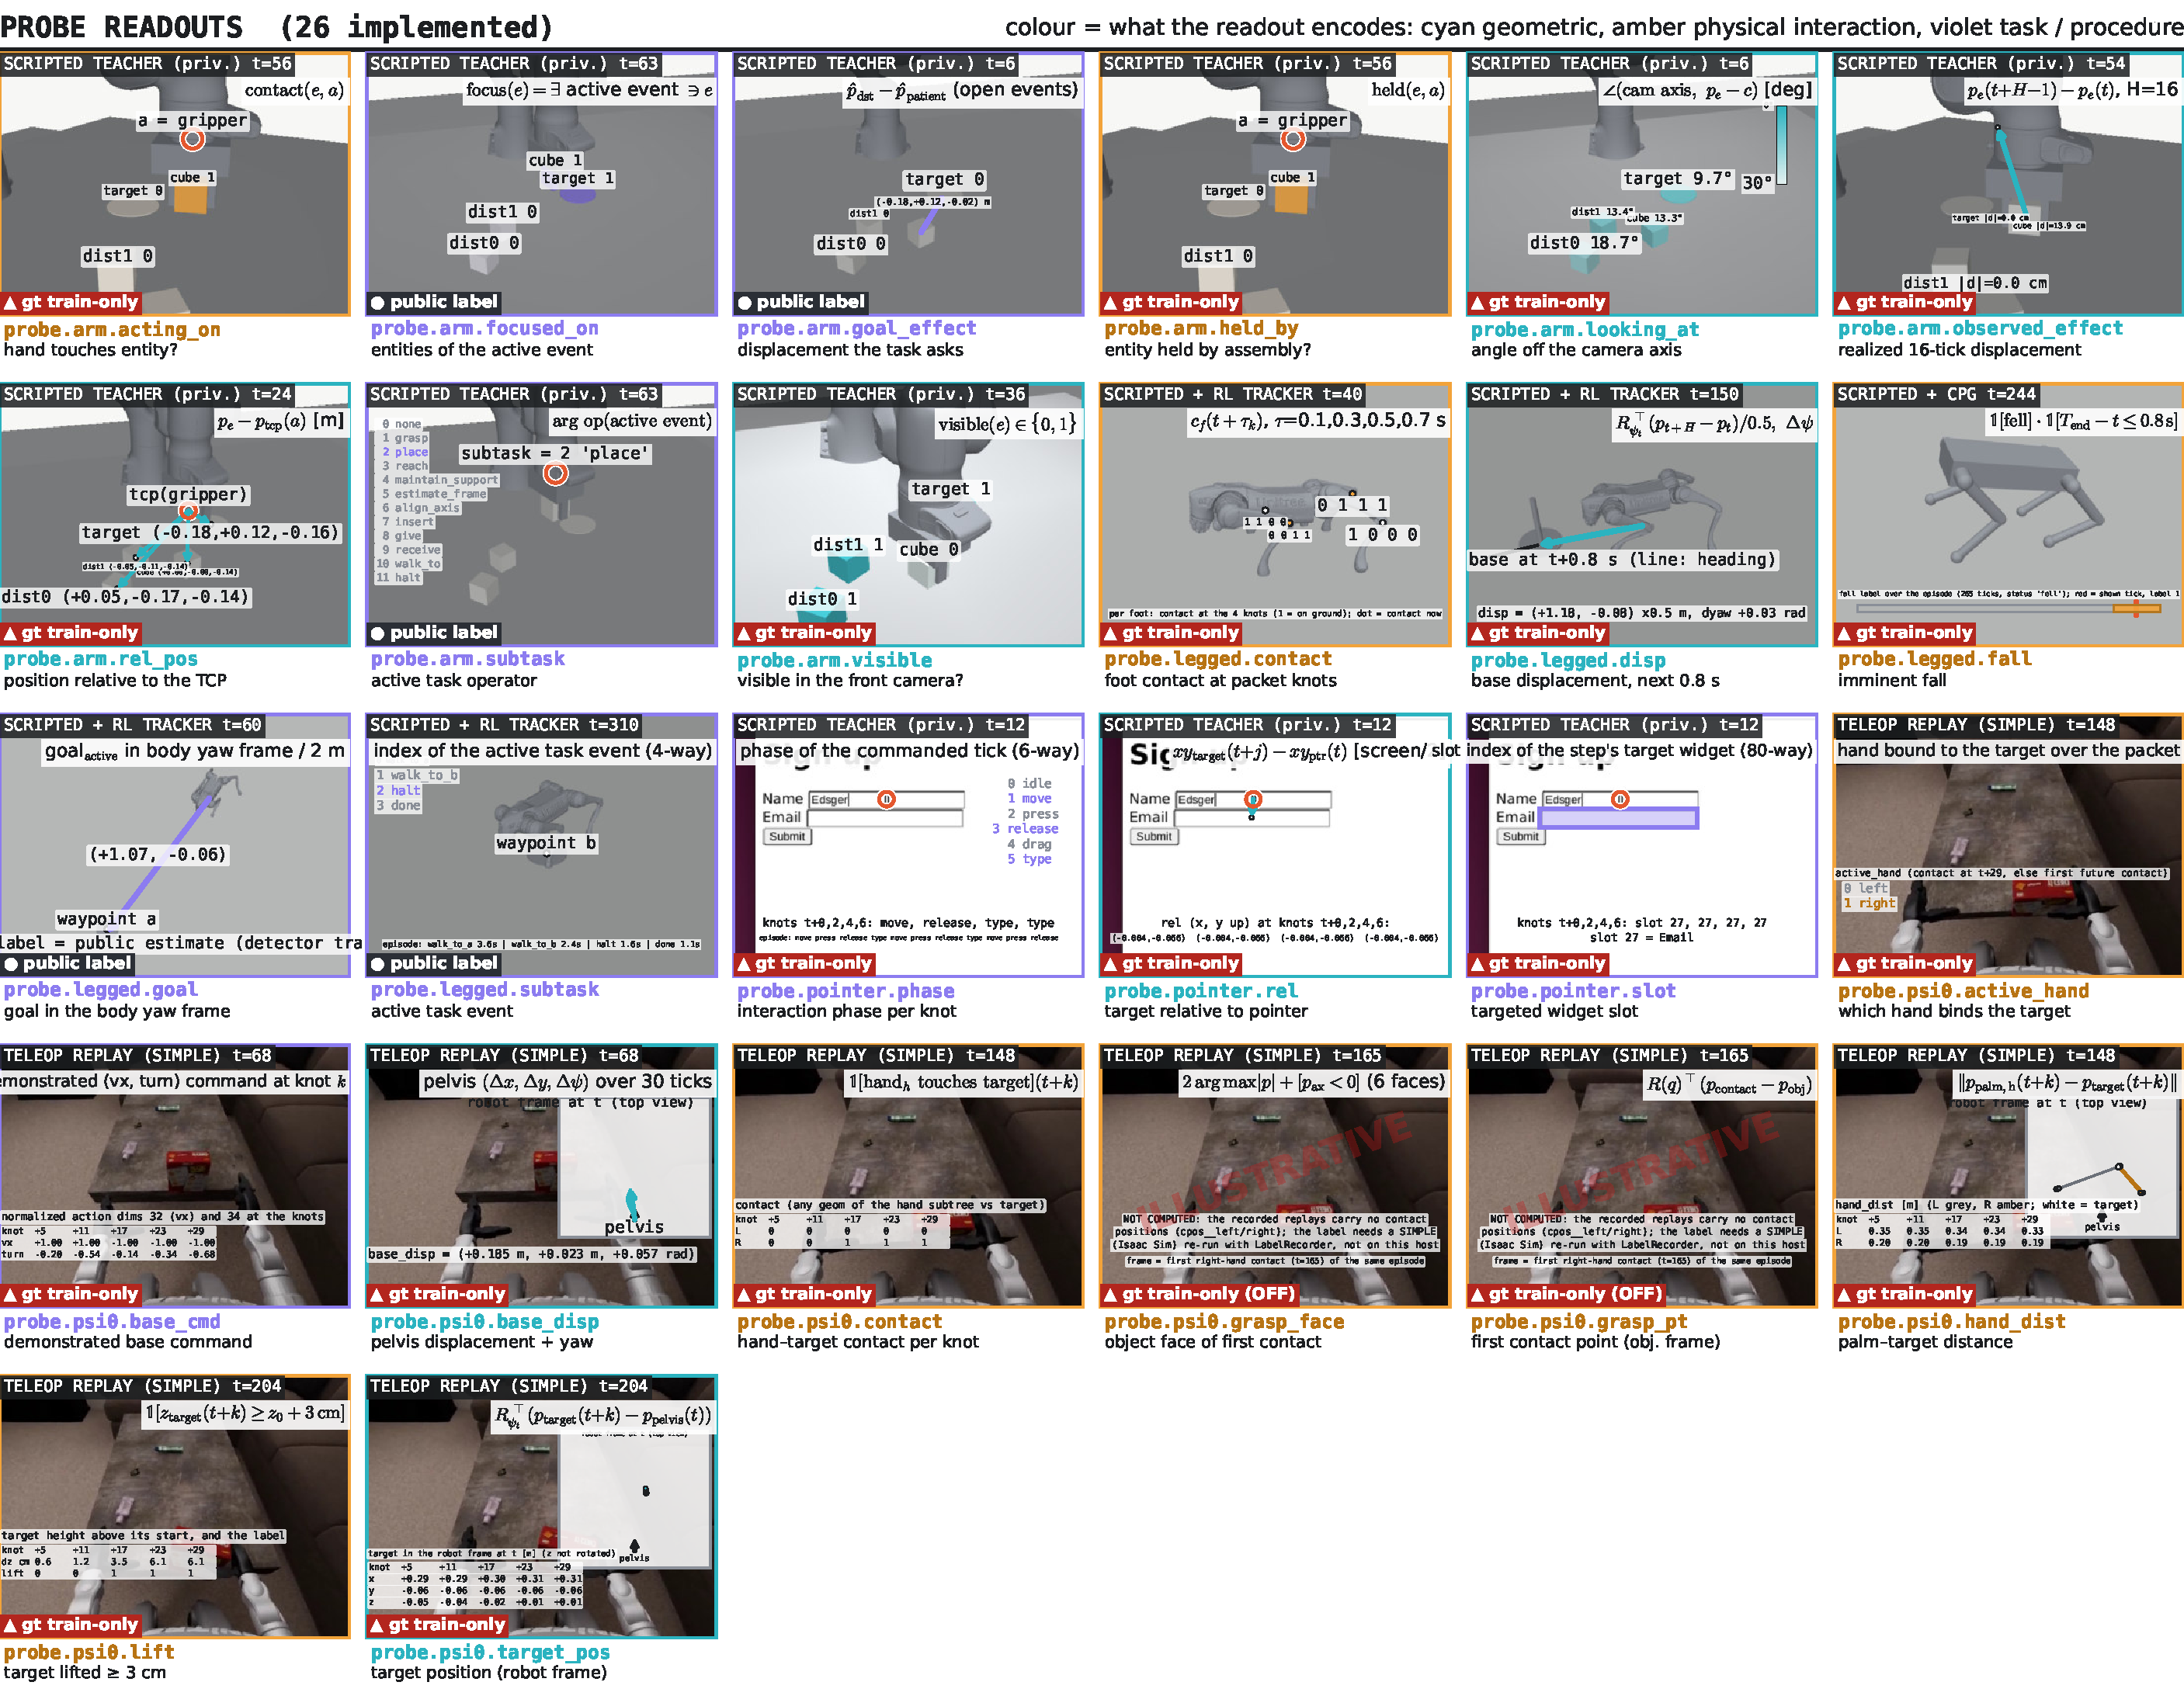
\includegraphics[width=\textwidth]{figures/factor_grid_p3.pdf}
\ContinuedFloat\captionsetup{font=footnotesize}\caption[]{\textbf{Every implemented relation factor} (continued, page 3/5). Badges, colours and marks as on the first page.}
\end{table*}
\begin{table*}[p]
\captionsetup{type=figure}
\centering
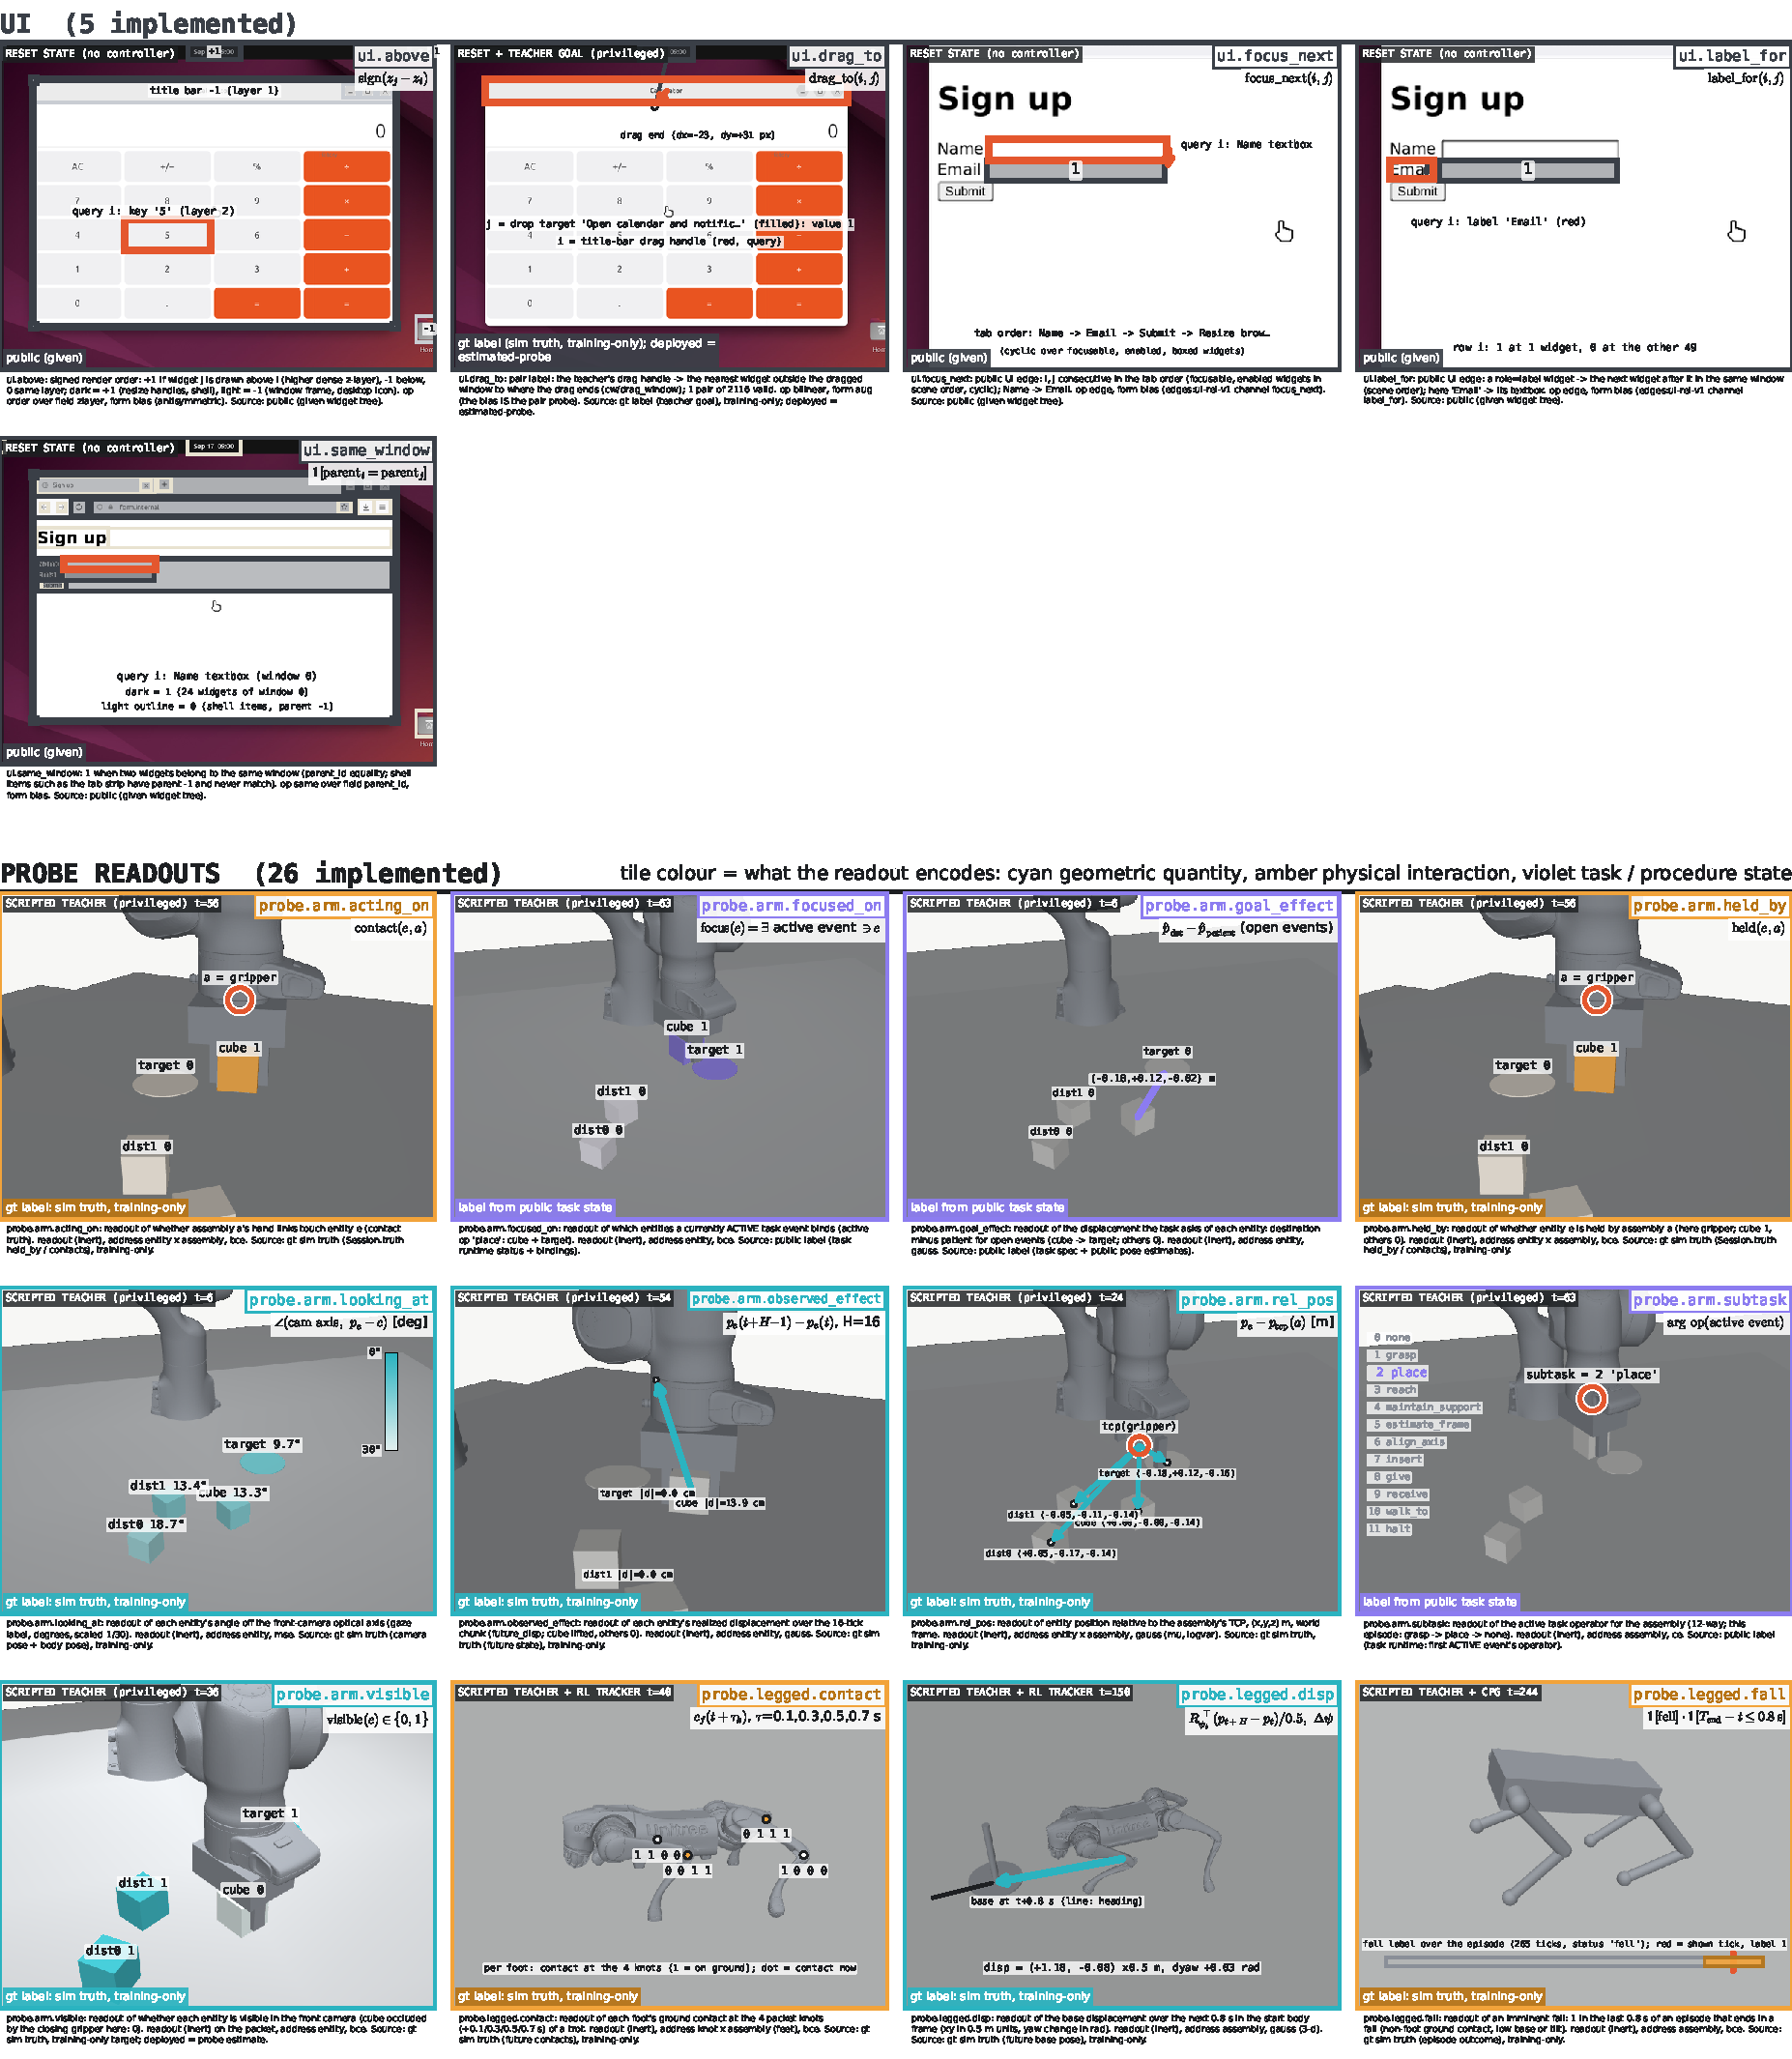
\includegraphics[width=\textwidth]{figures/factor_grid_p4.pdf}
\ContinuedFloat\captionsetup{font=footnotesize}\caption[]{\textbf{Every implemented relation factor} (continued, page 4/5). Badges, colours and marks as on the first page.}
\end{table*}
\begin{table*}[p]
\captionsetup{type=figure}
\centering
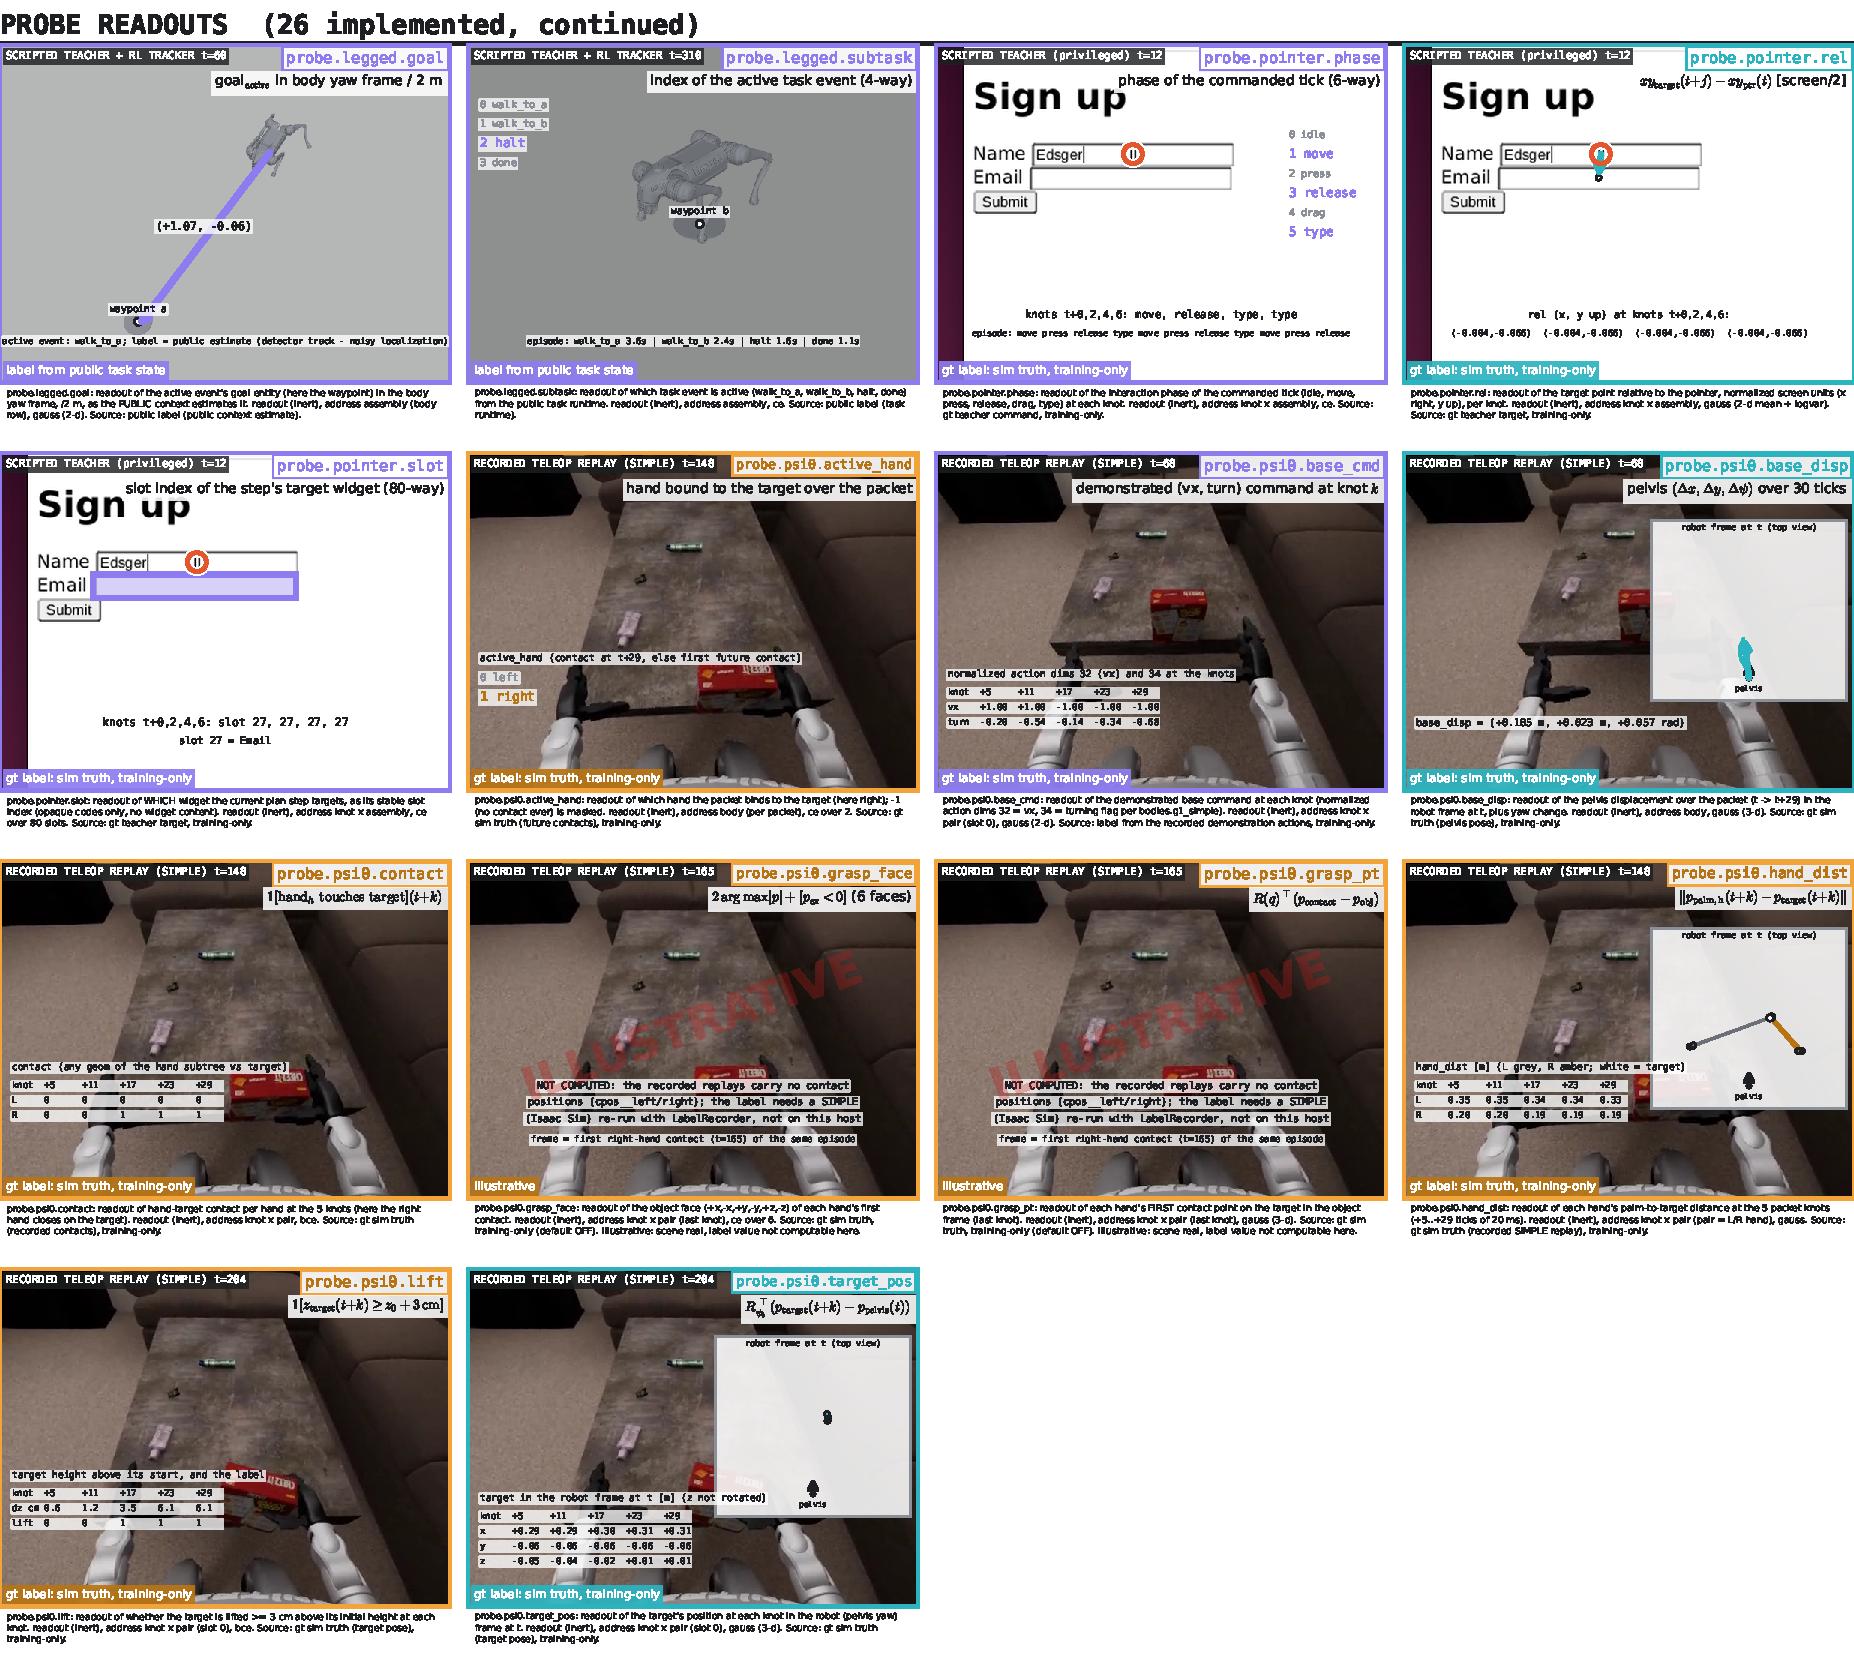
\includegraphics[width=\textwidth]{figures/factor_grid_p5.pdf}
\ContinuedFloat\captionsetup{font=footnotesize}\caption[]{\textbf{Every implemented relation factor} (continued, page 5/5). Badges, colours and marks as on the first page.}
\end{table*}
}
